\documentclass[sigconf,screen,review,anonymous]{acmart}

\usepackage{booktabs}
\usepackage{graphicx}
\usepackage{amsmath}
\usepackage{CJKutf8}
\usepackage{placeins}

\graphicspath{{../../figures/paper/}}
\renewcommand{\dbltopfraction}{0.9}
\renewcommand{\textfraction}{0.05}
\renewcommand{\floatpagefraction}{0.8}
\renewcommand{\dblfloatpagefraction}{0.8}
\setcopyright{none}
\settopmatter{printacmref=false}
\renewcommand\footnotetextcopyrightpermission[1]{}
\acmConference[ACM MM '26]{34th ACM International Conference on Multimedia}{November 10--14, 2026}{Rio de Janeiro, Brazil}
\acmYear{2026}

\title{Industrial Steam Prediction with Regularized Regression, Tree Ensembles, and Model Fusion}

% Anonymous review version required by the ACM MM 2026 main technical track.
% TODO(camera-ready): replace anonymous metadata only after acceptance instructions arrive.
\author{Anonymous Author(s)}

\begin{document}

\begin{abstract}
Industrial steam prediction from anonymized process measurements is a challenging soft-sensing problem: correlated variables favor regularization, nonlinear responses motivate tree ensembles, and model fusion helps only when base predictors provide complementary errors. We present a controlled empirical study using 38 anonymous features and a unified five-fold TimeSeriesSplit protocol. The study compares Ridge regression, XGBoost, gradient boosting, LightGBM, and random forests; evaluates feature selection and principal-component processing; analyzes Ridge regularization sensitivity; and tests weighted blending and stacking on an independent 481-sample fusion validation set. Best Ridge achieves the lowest cross-validation mean squared error (MSE), 0.1304, while tuning improves XGBoost to 0.1498 without surpassing the Ridge family. A 0.7/0.3 Ridge--XGBoost blend obtains an MSE of 0.1766 on the independent validation set, only about 0.19\% below Best Ridge, indicating a marginal numerical gain. SHAP analysis is restricted to Best XGBoost and reveals a concentrated global contribution profile. Prediction and residual diagnostics retain all validation samples and expose both accurate central predictions and substantial tail errors. The results demonstrate the competitiveness of regularized linear baselines under the evaluated setting.
\end{abstract}

\begin{CCSXML}
<ccs2012>
 <concept><concept_id>10010147.10010257</concept_id><concept_desc>Computing methodologies~Machine learning</concept_desc><concept_significance>500</concept_significance></concept>
 <concept><concept_id>10002950.10003705.10003707</concept_id><concept_desc>Mathematics of computing~Regression analysis</concept_desc><concept_significance>300</concept_significance></concept>
</ccs2012>
\end{CCSXML}
\ccsdesc[500]{Computing methodologies~Machine learning}
\ccsdesc[300]{Mathematics of computing~Regression analysis}
\keywords{industrial steam prediction, soft sensor, Ridge regression, XGBoost, model fusion, SHAP, time-series cross-validation}

\maketitle

\section{Introduction}
Industrial processes often contain quality, yield, or energy variables that are expensive, delayed, or impractical to measure online. Data-driven soft sensors estimate such targets from routinely acquired measurements and support monitoring and operational decisions. Process variables can be correlated, operating conditions can drift, responses can be nonlinear, and labels may be sparse or delayed. Reviews therefore emphasize validation design, model maintenance, and deployment reliability alongside predictive accuracy~\cite{kadlec2009softsensor,yeo2023jit,sheng2024review,perera2023ai_softsensor}.

Modern soft sensors include regularized linear models, tree ensembles, neural sequence models, and hybrids. Seq2Seq--LightGBM models have been studied for dynamic estimation~\cite{li2020seq2seq_lightgbm}; random forests have been deployed in an industrial debutanizer~\cite{botha2021industrial_softsensor}; and random-forest feature selection has been combined with deep learning for fermentation~\cite{hua2023rf_feature_selection}. Ensemble and multi-output designs further exploit complementary predictors or correlated outputs~\cite{wang2019two_layer_ensemble,pan2019ensemble_jit,wan2024wide_rf}. These studies motivate broad comparison, but model complexity alone does not guarantee better generalization.

Anonymous features impose a further constraint: without physical meanings, they cannot support claims about temperature, pressure, flow, or causal mechanisms. Evaluation must rest on reproducible predictive evidence. Principal-component analysis (PCA) and univariate selection can reduce dimensionality, but their value depends on the data and estimator~\cite{jolliffe2016pca,guyon2003feature_selection}. Hyperparameter optimization can likewise identify a numerical minimum without producing a practically meaningful gain.

Stacking~\cite{wolpert1992stacking} and weighted averaging can reduce error when base learners make complementary mistakes, as industrial ensemble soft sensors illustrate~\cite{wang2019two_layer_ensemble,pan2019ensemble_jit}. Fusion can also add complexity for negligible gain. It therefore requires an independent validation set, comparison with the strongest constituent model, and separation of weight-search scores from final held-out evaluation.

SHAP provides additive feature attributions~\cite{lundberg2017shap} and has been applied to tree-based and attention-based industrial soft sensors~\cite{cao2023interpretable_softsensor,cao2024informer_shap}. An attribution analysis explains only the model for which it was computed; here it is limited to Best XGBoost. Aggregate metrics also conceal tail behavior, motivating observed-versus-predicted and residual views.

Validation design connects these choices. Random folds can be optimistic when neighboring observations share temporal or operational structure, whereas ordered splits can expose distribution changes. The appropriate protocol depends on acquisition and deployment assumptions~\cite{bergmeir2012cv,bergmeir2018cv}. Row order is available here, but strict time semantics are not fully documented. We use TimeSeriesSplit as the primary protocol and KFold only to assess sensitivity; their difference does not establish that either splitter is universally preferable.

Five fold scores are not independent replications of the complete experiment, and their standard deviation is not a confidence interval. A single fusion-validation set supports descriptive comparison but cannot establish that a small difference will persist across datasets or operating periods. Accordingly, ``best'' denotes the lowest observed mean under the stated protocol, not statistically verified superiority.

The analysis concerns sensor-derived industrial data, model fusion, and interpretable prediction, topics adjacent to the conference's stated interests in sensor data, multimodal fusion, and interpretability. Because the dataset does not expose physical modalities, we make no stronger multimodality claim.

This paper studies industrial steam prediction from 38 anonymous features in a controlled pipeline. It compares regularized regression with four tree-model families under five-fold TimeSeriesSplit; evaluates full-feature Ridge, KBest20, PCA95, and Ridge regularization sensitivity; and tests weighted blending and stacking on an independent 481-sample set. Model-bounded SHAP analysis and uncensored residual diagnostics complement the performance results. The contribution is an evidence-aligned comparison of modeling choices rather than a new learning algorithm.

\section{Related Work}
\subsection{Industrial Soft Sensing and Process Prediction}
Data-driven soft sensors map accessible process measurements to difficult-to-measure variables~\cite{kadlec2009softsensor}. Recent reviews highlight local adaptation, distribution shift, and reliable deployment as continuing issues~\cite{yeo2023jit,sheng2024review,perera2023ai_softsensor}. Applications range from distillation and fermentation~\cite{botha2021industrial_softsensor,hua2023rf_feature_selection} to dynamic and multi-output prediction~\cite{li2020seq2seq_lightgbm,wan2024wide_rf}. Engineering studies have also used XGBoost for wind-power prediction and cross-dimensional feature fusion for remaining-life estimation~\cite{wang2023zju_wind_xgboost,zhang2025zju_feature_fusion}. Our study differs by holding the validation protocol fixed while comparing linear and tree estimators on anonymous industrial measurements.

\subsection{Regularization, Tree Ensembles, and Fusion}
Ridge regression stabilizes correlated linear estimates through an $\ell_2$ penalty~\cite{hoerl1970ridge}. XGBoost~\cite{chen2016xgboost}, LightGBM~\cite{ke2017lightgbm}, random forests~\cite{breiman2001randomforest}, and gradient boosting~\cite{friedman2001gbdt} offer nonlinear alternatives. Stacked generalization combines base learners through a meta-model~\cite{wolpert1992stacking}; recent process and engineering applications show the practical appeal of ensemble construction~\cite{wang2019two_layer_ensemble,hu2025zju_stacking}. We focus on whether that additional complexity yields a meaningful held-out gain over Best Ridge.

\subsection{Interpretability and Validation}
SHAP unifies additive feature attribution methods~\cite{lundberg2017shap}. XGBoost--SHAP and related approaches have supported engineering prediction and nonlinear-effect analysis~\cite{chen2023zju_xgboost_shap,lu2025zju_xgboost_shap}. Mean absolute SHAP values quantify global contribution magnitude, not direction or causality. Validation choices are similarly contextual: cross-validation for ordered or autoregressive observations requires assumptions about dependence and prediction use~\cite{bergmeir2012cv,bergmeir2018cv}. We therefore treat KFold comparison as sensitivity analysis, not proof that either splitter is universally correct.

\section{Problem Setup and Data}
The training data contain 2,888 rows, 38 anonymous inputs $V0$--$V37$, and a continuous target. The unlabeled test set contains 1,925 rows and is not used to report error metrics. For sample $i$, $\mathbf{x}_i\in\mathbb{R}^{38}$ and $y_i\in\mathbb{R}$; a predictor $f$ returns $\hat y_i=f(\mathbf{x}_i)$. Surface-level checks found no missing values, duplicate rows, or infinite values in the training data. Because metadata do not establish the physical meaning of the variables or fully certify temporal semantics, we avoid process-specific causal claims.

Figure~\ref{fig:target} shows the complete target distribution. The mean is 0.126 and the median is 0.313; observations extend into both tails. The histogram supplies scale context for later squared and absolute errors rather than evidence about model performance.

\begin{figure}[t]
\centering
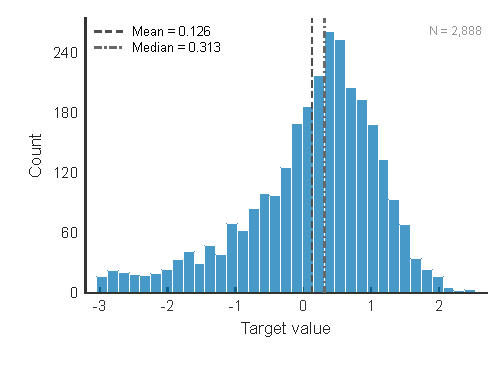
\includegraphics[width=\columnwidth]{fig1_target_distribution.pdf}
\caption{Distribution of the industrial steam target. Bins follow the Freedman--Diaconis rule; all 2,888 samples are retained.}
\Description{Histogram of 2,888 target values with dashed mean and dash-dotted median reference lines. The distribution has a dense central region and observations in both tails.}
\label{fig:target}
\end{figure}

\section{Methodology}
\subsection{Predictive Models}
Inputs are standardized before Ridge fitting. Ridge minimizes
\begin{equation}
\|\mathbf{y}-\mathbf{X}\boldsymbol{\beta}\|_2^2+\alpha\|\boldsymbol{\beta}\|_2^2,
\end{equation}
where $\alpha$ controls shrinkage. We compare ten settings from 0.01 to 100: 0.01, 0.1, 0.5, 1, 2, 5, 10, 20, 50, and 100. Tree baselines are XGBoost, GBDT, LightGBM, and Random Forest. Best XGBoost uses 300 trees, learning rate 0.05, maximum depth 2, subsample 0.8, column subsample 1.0, and random seed 42.

\subsection{Feature Processing and Fusion}
Ridge is evaluated with all 38 inputs, KBest retaining 20 features, and PCA retaining 95\% cumulative explained variance. For fusion, Best Ridge and Best XGBoost predictions are combined as
\begin{equation}
\hat y_{\mathrm{blend}}=0.7\hat y_{\mathrm{Ridge}}+0.3\hat y_{\mathrm{XGB}}.
\end{equation}
Stacking is included as a second fusion baseline. Final fusion claims use only the independent 481-sample validation set; the more optimistic value observed during weight search is excluded.

\subsection{Model-Bounded Explanation}
We compute global mean absolute SHAP values only for Best XGBoost. These values summarize attribution magnitude. They do not encode positive or negative effects, causal influence, uncertainty, or statistical significance, and they do not explain Weighted Blend.

\section{Experiments}
\subsection{Protocols and Metrics}
The main comparison uses five-fold TimeSeriesSplit; KFold is retained only as a sensitivity check because strict temporal semantics are not fully documented. The metrics are MSE, RMSE, MAE, and $R^2$, with RMSE defined as the mean of fold-level square-root MSE values. Fold standard deviations describe variability rather than confidence intervals. The fusion comparison uses a separate fixed validation set of 481 samples and is not directly comparable with the cross-validation means.

Every entry in the principal comparison uses the same ordered five-fold partitioning rule. Scaling, KBest, and PCA are fitted within their training pipelines so held-out folds do not determine preprocessing. Hyperparameter results are reported at their observed cross-validation means and interpreted relative to neighboring configurations.

MSE is the primary ranking metric; RMSE restores the target scale, MAE is less dominated by large residuals, and $R^2$ measures explained variation relative to a constant-mean predictor. All values come from frozen result tables shared by the figures and tables. The unlabeled test set is excluded from metric reporting, the final fusion result is kept separate from its weight-search score, and no repeated independent fusion trials are available. Comparisons are therefore descriptive, with no significance inference.

\subsection{Model Comparison}
Figure~\ref{fig:model} and Table~\ref{tab:main} summarize the main protocol. Best Ridge has the lowest mean MSE, 0.1304, but ordinary Ridge is very close at 0.1306. Tuning improves XGBoost from 0.1542 to 0.1498, yet it remains behind both Ridge variants.

Moving from $\alpha=1$ in the baseline pipeline to $\alpha=5$ changes Ridge mean MSE by roughly two ten-thousandths at the displayed precision. Tuning XGBoost reduces mean MSE by about 0.0044 and improves the other metrics, but it does not close the gap to Ridge.

Fold standard deviations in Figure~\ref{fig:model} are of comparable order across models. Best Ridge and Ridge are numerically close; the error bars do not establish equivalence or significance.

\begin{figure}[t]
\centering
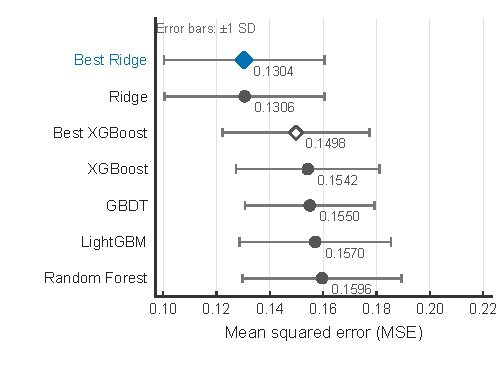
\includegraphics[width=\columnwidth]{fig2_model_performance.pdf}
\caption{Model MSE under five-fold TimeSeriesSplit. Error bars denote $\pm1$ fold standard deviation.}
\Description{Ranked dot-whisker plot for seven models. Best Ridge and Ridge are nearly coincident at the lowest mean MSE; tree models have higher mean errors.}
\label{fig:model}
\end{figure}

\begin{table}[t]
\caption{Five-fold TimeSeriesSplit performance.}
\label{tab:main}
\centering\small
\begin{tabular}{lrrrr}
\toprule
Model & MSE & RMSE & MAE & $R^2$\\
\midrule
Best Ridge & \textbf{.1304} & \textbf{.3593} & \textbf{.2639} & \textbf{.8525}\\
Ridge & .1306 & .3595 & .2643 & .8523\\
Best XGBoost & .1498 & .3858 & .2888 & .8261\\
XGBoost & .1542 & .3915 & .2952 & .8203\\
GBDT & .1550 & .3927 & .2964 & .8207\\
LightGBM & .1570 & .3950 & .2990 & .8186\\
Random Forest & .1596 & .3981 & .2997 & .8164\\
\bottomrule
\end{tabular}
\end{table}

\subsection{Feature and Regularization Sensitivity}
Figure~\ref{fig:feature}a and Table~\ref{tab:feature} show that full-feature Ridge performs best under the current setting. KBest20 and PCA95 do not improve the error, but this result does not generalize to feature selection as a whole. Figure~\ref{fig:feature}b shows a broad shallow region: $\alpha=5$ produces the lowest observed mean MSE of 0.130369, only slightly below neighboring settings. Error rises more visibly at 20, 50, and 100.

KBest20 discards nearly half of the anonymous inputs and raises mean MSE from 0.1306 to 0.1389. PCA95 increases it further to 0.1681. Because Ridge already shrinks correlated coefficients, aggressive projection or univariate screening may remove weak but jointly useful information. That explanation is plausible rather than proven: anonymous variables prevent a process-level account, and different selection criteria or dimensionalities might behave differently. The defensible conclusion is therefore restricted to the tested KBest20 and PCA95 configurations.

The regularization curve also clarifies why the label ``Best Ridge'' should be used cautiously. Mean MSE changes little between 0.01 and 10, reaching a shallow minimum at 5. At stronger regularization, coefficient shrinkage eventually introduces enough bias for the error to rise. This curve favors a stable interval of reasonable choices over a narrative centered on a uniquely correct hyperparameter.

\begin{figure*}[t]
\centering
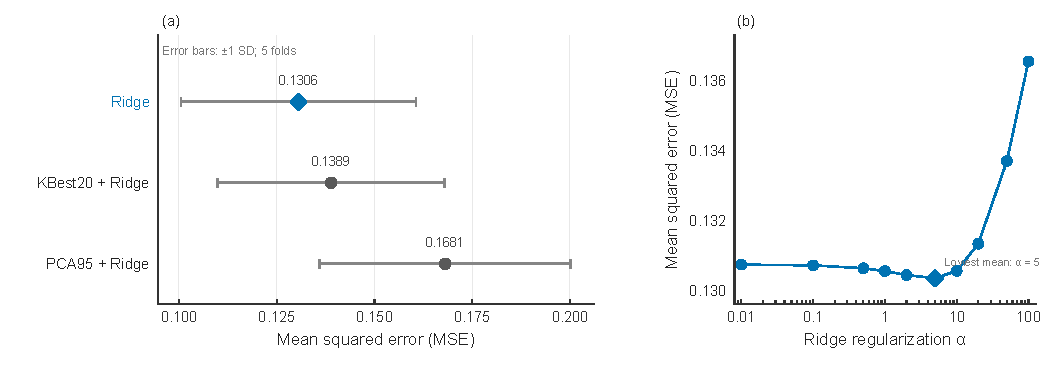
\includegraphics[width=\textwidth]{fig3_feature_ridge_sensitivity.pdf}
\caption{Feature-processing comparison and Ridge regularization sensitivity. (a) Error bars are $\pm1$ fold SD. (b) Mean MSE only; $\alpha=5$ is a shallow numerical optimum.}
\Description{Two panels: a dot-whisker comparison of three Ridge input strategies, and a log-alpha sensitivity curve with ten points. Full-feature Ridge is lowest; the curve is nearly flat around alpha 5 and rises at large alpha.}
\label{fig:feature}
\end{figure*}

\begin{table}[t]
\caption{Ridge feature-processing comparison.}
\label{tab:feature}
\centering\small
\begin{tabular}{lrrrr}
\toprule
Method & MSE & RMSE & MAE & $R^2$\\
\midrule
Ridge & \textbf{.1306} & \textbf{.3595} & \textbf{.2643} & \textbf{.8523}\\
KBest20 + Ridge & .1389 & .3711 & .2736 & .8424\\
PCA95 + Ridge & .1681 & .4085 & .3116 & .8074\\
\bottomrule
\end{tabular}
\end{table}

\section{Results}
\subsection{Fusion Performance}
On the independent validation set, Weighted Blend reaches MSE 0.176594 compared with 0.176921 for Best Ridge (Figure~\ref{fig:fusion} and Table~\ref{tab:fusion}). The relative reduction is approximately 0.19\%, a marginal numerical improvement. Stacking is slightly worse than Best Ridge, whereas Best XGBoost is clearly worse.

All four metrics tell the same descriptive story. Weighted Blend has RMSE 0.4202, MAE 0.2870, and $R^2$ 0.8190; Best Ridge has 0.4206, 0.2882, and 0.8186. Stacking yields MSE 0.1790, and Best XGBoost reaches 0.1968. The blend therefore preserves the strong Ridge component while receiving a small correction from XGBoost, but the correction is insufficient to create a practically large separation. A deployment decision should weigh this small gain against the cost of maintaining two models and a fixed combination rule.

The absolute fusion-set errors are higher than the five-fold means in Table~\ref{tab:main}, but the sample set and evaluation protocol differ. Table~\ref{tab:fusion} therefore supports comparisons among its four rows only.

\begin{figure}[t]
\centering
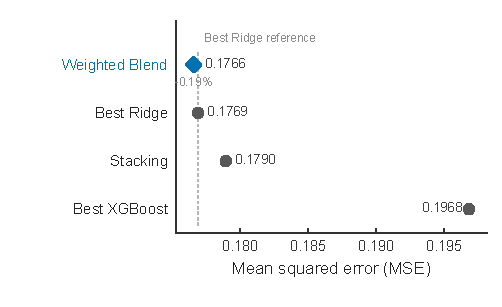
\includegraphics[width=\columnwidth]{fig4_fusion_comparison.pdf}
\caption{MSE on the independent fusion validation set. Weighted Blend and Best Ridge are numerically very close.}
\Description{Ranked dot plot of four models on a continuous MSE axis. Weighted Blend is slightly left of the Best Ridge reference line; Best XGBoost is farthest right.}
\label{fig:fusion}
\end{figure}

\begin{table}[t]
\caption{Independent fusion-validation performance.}
\label{tab:fusion}
\centering\small
\begin{tabular}{lrrrr}
\toprule
Model & MSE & RMSE & MAE & $R^2$\\
\midrule
Weighted Blend & \textbf{.1766} & \textbf{.4202} & \textbf{.2870} & \textbf{.8190}\\
Best Ridge & .1769 & .4206 & .2882 & .8186\\
Stacking & .1790 & .4230 & .2905 & .8166\\
Best XGBoost & .1968 & .4436 & .3032 & .7983\\
\bottomrule
\end{tabular}
\end{table}

\subsection{Global SHAP Importance}
Figure~\ref{fig:shap} reports the top 15 features for Best XGBoost. V0 (0.329) and V1 (0.179) dominate, followed by a rapid decrease. Only aggregated mean absolute SHAP values are available, so the figure reports contribution magnitude without per-sample distributions, directions, or uncertainty bars.

The head concentration suggests that the tree branch obtains much of its predictive contribution from a small subset of anonymous inputs. It does not establish that the remaining variables are useless to Ridge or to the final blend, because feature use and attribution are model dependent. Nor can V0 or V1 be assigned a physical mechanism without metadata. The result is therefore most useful as an auditing signal: future data documentation and robustness checks should prioritize the provenance and stability of these high-contribution variables.

\begin{figure}[t]
\centering
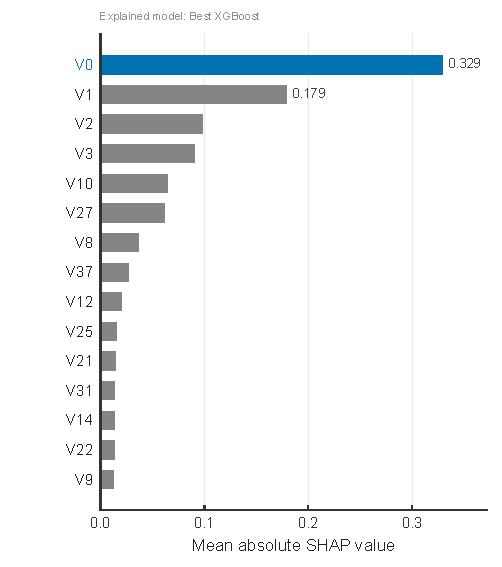
\includegraphics[width=\columnwidth]{fig5_shap_importance.pdf}
\caption{Global mean absolute SHAP importance for Best XGBoost.}
\Description{Horizontal bars for the top 15 features. V0 is longest, V1 is second, and importance decreases sharply thereafter.}
\label{fig:shap}
\end{figure}

\begin{figure*}[!t]
\centering
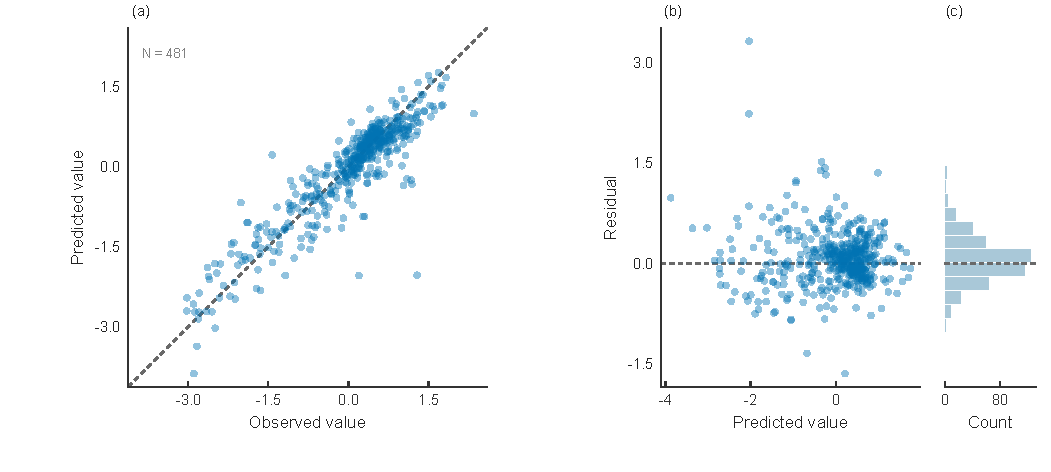
\includegraphics[width=\textwidth]{fig6_prediction_diagnostics.pdf}
\caption{Weighted Blend diagnostics on the independent fusion validation set. All 481 samples are retained.}
\Description{Three panels show observed versus predicted values with an identity line, residual versus predicted values with a zero line, and a horizontal residual histogram sharing the same residual range. Large residuals remain visible.}
\label{fig:diagnostics}
\end{figure*}

\subsection{Prediction Diagnostics}
Figure~\ref{fig:diagnostics} retains all 481 validation samples. Weighted Blend obtains MSE 0.176594, RMSE 0.420, MAE 0.287, and $R^2$ 0.819. Most predictions track observations, but several large deviations remain. Residuals occur on both sides of zero and include a longer positive tail; the histogram supplies tail context without imposing a fitted distribution.

The identity-scaled observed-versus-predicted panel prevents aspect-ratio distortion from making the fit look artificially tight. The residual panel shows both underestimation and overestimation relative to the zero line, while the subordinate histogram confirms a concentrated center accompanied by tails. No samples are clipped, removed, or separately relabeled. This matters because the squared-error metric is particularly sensitive to the visible large residuals; suppressing them would disconnect the figure from the reported MSE.

\section{Discussion}
The central result is the competitiveness of regularized linear prediction under the evaluated setting. Correlation among anonymous inputs can make Ridge effective even when nonlinear alternatives are available. Its tuning gain is tiny, supporting a stable regularization region rather than a uniquely superior $\alpha$. Neither KBest20 nor PCA95 helps in this experiment.

From an industrial modeling perspective, this outcome argues for complexity-aware baselines. A compact linear model is easier to retrain, inspect, and deploy, and its behavior under correlated predictors is well understood. Tree ensembles remain valuable when nonlinear interactions dominate, but their flexibility is not itself evidence of superior generalization. Similar lessons motivate careful comparisons in practical soft-sensor systems, including interpretable tree ensembles and recent engineering fusion studies~\cite{cao2023interpretable_softsensor,chen2023zju_xgboost_shap,hu2025zju_stacking}.

The fusion experiment illustrates why protocol separation matters. The lower search-stage error is excluded from the final claim. On the independent set, Weighted Blend improves on Best Ridge by only about 0.19\%; this small gain must be weighed against the cost of maintaining two models and a fixed combination rule.

\FloatBarrier

The validation sensitivity result reinforces this caution. Best Ridge yields MSE 0.130369 with TimeSeriesSplit and 0.112940 with KFold. The latter is lower, but the difference cannot prove that KFold is more appropriate; it reveals dependence on the splitting assumption. Stronger temporal metadata and repeated evaluations would be needed for a firmer conclusion.

The SHAP ranking shows that Best XGBoost relies heavily on a small feature head, but anonymous names prevent physical interpretation and mean absolute values omit direction. Residual diagnostics complement that branch-specific view by showing tail risk in the final blend. Limitations include one dataset, anonymous variables, uncertain temporal semantics, no repeated independent trials, and no significance testing.

These limitations define concrete next steps. Time stamps and operating-regime labels would enable blocked or rolling-origin evaluations tied to deployment conditions. Repeated outer validation could quantify uncertainty in the small fusion difference. Drift monitoring could test whether V0 and V1 remain dominant for Best XGBoost over time, and process metadata could turn anonymous associations into engineering hypotheses. None of these extensions should retroactively strengthen the claims supported by the present frozen results.

\section{Conclusion}
Best Ridge leads the seven models under the ordered five-fold protocol; XGBoost tuning improves its tree baseline without overtaking Ridge. Full-feature Ridge outperforms KBest20 and PCA95 in this experiment, and $\alpha=5$ is a shallow numerical optimum. On an independent 481-sample set, a 0.7/0.3 Ridge--XGBoost blend improves MSE over Best Ridge by only about 0.19\%. Best-XGBoost SHAP importance is concentrated in a few features, and complete-sample diagnostics expose residual tails. These findings favor protocol-aligned, dataset-bounded conclusions.

\begin{CJK*}{UTF8}{gbsn}
\bibliographystyle{ACM-Reference-Format}
\bibliography{references}
\end{CJK*}

\end{document}
